	\documentclass[a4paper,12pt]{exam}

%PACOTES

\usepackage[brazil]{babel}
\usepackage[utf8]{inputenc}
%\usepackage[latin1]{inputenc}
\usepackage[T1]{fontenc}
\usepackage{tikz}
\usepackage{pgfkeys}
\usepackage{svg}
%\usepackage[siunitx, RPvoltages]{circuitikz}
%\usemodule[circuitikz]
 
%FONTES-------------------------------------------------
\usepackage{helvet}
\renewcommand{\familydefault}{\sfdefault}
%\usepackage{gfsartemisia-euler}
%\renewcommand{\familydefault}{pzc}
%-------------------------------------------------------

\usepackage[onehalfspacing]{setspace}
\usepackage{fourier}
\usepackage[lmargin=1.9cm,rmargin=1.6cm,tmargin=2cm,bmargin=3cm]{geometry}
\usepackage[onehalfspacing]{setspace}
\usepackage{amsmath,amssymb}%Expressoes matem�ticas e s�mbolos
\RequirePackage{amssymb, amsfonts, amsmath, latexsym, verbatim, xspace, setspace}
\usepackage{multicol}% M�ltiplas colunas
\usepackage{multirow}% permite mesclar c�lulas de modo horizontal
\usepackage{array}%para tabelas
\usepackage{ragged2e}%alinhamento
\usepackage{graphicx}%Para inserir imagens
\usepackage{pdflscape}%Permite mudar a orientacao da pagina
\usepackage{epstopdf} %converte figs eps em figs pdf
\usepackage{booktabs}%tabelas
\usepackage{pdfpages}%Permite incluir arquivos pdf
\usepackage[sort&compress,square,comma, authoryear]{natbib}%Referencias
\usepackage[colorlinks=true,urlcolor=magenta,citecolor=red,linkcolor=blue,bookmarks=true]{hyperref}%Links e cita��es
\usepackage{enumerate}%enumeracao
\usepackage{enumitem}%enumeracao
\usepackage{pgf}
\usepackage{pgfpages}%Bordas das p�ginas
\usepackage[
    per-mode=fraction,
    quotient-mode=fraction,
    ]{siunitx}
\usepackage{import}
\usepackage{color,xcolor}
\usepackage{cancel}
\usepackage{fancybox}

%CONFIGURA��ES DA CLASSE EXAM

\renewcommand{\thequestion}{\bf \arabic{question}}
\pointpoints{ponto}{pontos}
\pointformat{\bf \small (\thepoints)}
\renewcommand{\choicelabel}{\bf \thechoice)}
\renewcommand{\solutiontitle}{{\bf Resposta: \enspace}}

\CorrectChoiceEmphasis{\color{red} \bf}
\SolutionEmphasis{\small \color{red}}

\everymath{\displaystyle} %deixa as equa��es do mesmo tamanho da letra normal
\addpoints %Necess�rio para exibir pontua��o no cabe�alho
\sisetup{output-decimal-marker = {,}}

%BORDA DA P�GINA
\pgfpagesdeclarelayout{boxed}
{
	\edef\pgfpageoptionborder{3pt}
}
{
	\pgfpagesphysicalpageoptions
	{%
		logical pages=1,%
	}
	\pgfpageslogicalpageoptions{1}
	{
		border code=\pgfsetlinewidth{0.5mm}\pgfstroke,%
		border shrink=\pgfpageoptionborder,%
		resized width=.95\pgfphysicalwidth,%
		resized height=.95\pgfphysicalheight,%
		center=\pgfpoint{.5\pgfphysicalwidth}{.5\pgfphysicalheight}%
	}%
}
\pgfpagesuselayout{boxed}
\setlength{\parindent}{.1cm}


  
  
  
  
  
  
  
  


	% EQUAÇÕES

\newcommand{\Eel}{$E=k\times\frac{\left| Q  \right|}{\left( d \right)^{2}}$} % Campo Elétrico
\newcommand{\Fel}{$F_e=k\times\frac{\left| Q \times q \right|}{\left( d \right)^{2}}$} % Força Elétrica
\newcommand{\Vm}{$\frac{\Delta S}{\Delta T}$}

% CONSTANTES

\newcommand{\cteK}{$k=\SI{9e9}{\newton\meter^2\per\coulomb^2}$} % Constante eletrostática no vácuo.

% UNIDADES

\newcommand{\uVmms}{\si{\meter\per\second}} % metros por segundo
\newcommand{\uVmkmh}{\si{\kilo\meter\per\hour}} % quilômetros por hora

	% ALTERAR

	\newcommand{\serie}{3° Ano} %Ex.: 1° Ano, 2° Ano, 3° Ano
	\newcommand{\data}{29/09/2021} %Ex.: today ou {\rule{1cm}{.3mm} /\rule{1cm}{.3mm} /\rule{1cm}{.3mm }
	\newcommand{\questaopt}{20} % Pontos por questão
	\newcommand{\duracao}{50 minutos}
	\printanswers %EXIBE AS RESPOSTAS E SOLUÇÕES
	
	\begin{document}
		
	   % % Especificações da prova

\newcommand{\orgao}{Secretaria da Educação do Estado do Ceará - SEDUC/CE}
\newcommand{\escola}{EEM Professora Francisca Linhares de Sousa}
\newcommand{\disciplina}{Física}
\newcommand{\professor}{Franklin Rios}
\newcommand{\prova}{\small{Lista de Exercícios}}
\newcommand{\conteudo}{Eletrostática}

\newcommand{\logofl}{
\includegraphics[width=2.5cm]{secoes/imagens/LogoFL.pdf}}
\newcommand{\logogov}{
\includegraphics[width=3cm]{secoes/imagens/LogoGov2.pdf}}

\begin{minipage}[c][1.8cm][c]{7cm}\hspace{-2cm}
	
%Tabela Cabeçalho
\hspace{-1.5cm}
\fbox{\fbox{\parbox{19.5cm}{\centering {
\hspace{-.1cm}
\begin{tabular}{lllrll}\hspace{.5cm}
	\\
\multirow{3}{*}{\logofl} \hspace{1cm} & \multicolumn{4}{l}{\textbf{\escola}}                           &\hspace{.1cm} \multirow{3}{*}{\logogov} \\
                         & \textbf{Disciplina: }& \disciplina & \textbf{Professor: } & \professor &                   \\
                         & \textbf{Série: }      & \serie      &  \textbf{Data: } & \data   \vspace{.3cm}    &         \\
\multicolumn{6}{c}{\large \textbf{\prova}}  \vspace{.1cm}  \\
\multicolumn{6}{c}{\large \textbf{\conteudo}}  \vspace{.2cm} 
\end{tabular}
}}}}

\end{minipage} 

\vspace{2cm}

%=========================================================
%------------Cabeçalho da Segunda página
%=========================================================

\pagestyle{headandfoot}%{head}%empty
\firstpageheader{}{}{}
\runningheader{\prova}{}{\disciplina}
\runningheadrule
\firstpagefooter{}{}{}
\runningfooter{}{Bons Estudos!}{Pág. \thepage\ de \numpages}
\runningfootrule
%======================================================== %CABEÇALHO LISTAS
%	    \input{secoes/cabBim} %CABEÇALHO PROVAS BIMESTRAIS
%	    \vspace{0.15cm}
\fbox{\fbox{\parbox{16.2cm}{\centering { \vspace{.2cm}{\bf \large Instruções para a prova}
	\begin{itemize}
		\item {\small Esta prova contém {\bf \numpages} página(s), incluindo esta capa, {\bf \numquestions} questões e vale {\bf 									\numpoints} pontos.}
		\item Confira se a quantidade e a ordem das questões estão de acordo com a instrução anterior. 
		\item Para cada questão são apresentadas \textbf{5} opções. Apenas uma responde corretamente a questão.
		\item O tempo disponível para realização dessa prova é de \textbf{\duracao}.
		\item As equações e constantes para a prova estão dadas nas questões.
		
		\end{itemize}
}}}}
\vspace{0.5cm}\\
\rule{17cm}{.03cm} %INSTRUÇÕES 
	 
	\begin{questions} %INICIA O AMBIENTE DE QUESTÕES
				
					%QUESTÃO - Cód.: TF1p0q01

\question [\questaopt] Um pescador encontrou um tesouro e o enterrou 
em um terreno cercado de sua propriedade. Para que ficasse fácil localizar 
o tesouro a qualquer momento, ele fez um esboço do terreno, associando
a ele um sistema de eixos cartesianos. Assim, ele mediu e marcou os
valores indicados na figura.

\begin{center}
	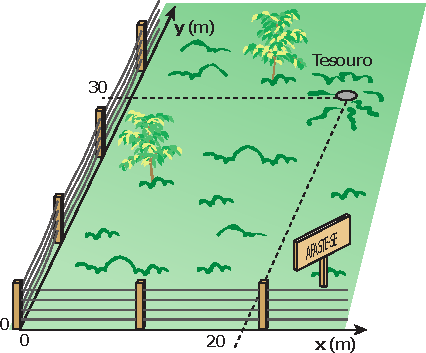
\includegraphics[width=0.4\linewidth]{questoes/imagens/TF1p01q01}
\end{center}



\begin{parts}

	\part Qual a abscissa do local em que está enterrado o tesouro?
	\part Qual a ordenada do local em que está enterrado o tesouro?

\end{parts}


%--------------------------SOLUÇÃO---------------------------------------

	\begin{solution}
		
	(a) 20 m; \\
	(b) 30 m.
		
	\end{solution}


					
    \end{questions}
	
\end{document}
